\documentclass[11pt]{scrartcl}
\usepackage{graphicx}
\graphicspath{{./}}
\usepackage[sexy]{evan}
\usepackage[normalem]{ulem}
\usepackage{hyperref}
\usepackage{mathtools}
\usetikzlibrary{calc}
\hypersetup{
    colorlinks=true,
    linkcolor=blue,
    filecolor=magenta,      
    urlcolor=cyan,
    pdfpagemode=FullScreen,
    }

\renewcommand{\dangle}{\measuredangle}

\renewcommand{\baselinestretch}{1.5}

\addtolength{\oddsidemargin}{-0.4in}
\addtolength{\evensidemargin}{-0.4in}
\addtolength{\textwidth}{0.8in}
% \addtolength{\topmargin}{-0.2in}
% \addtolength{\textheight}{1in} 


\setlength{\parindent}{0pt}

\usepackage{pgfplots}
\pgfplotsset{compat=1.15}
\usepackage{mathrsfs}
\usetikzlibrary{arrows}

\title{Length Bashing in OSN}
\author{Azzam (IG: haxuv.world)}
\date{\today}

\begin{document}
\maketitle

\renewcommand*\contentsname{Daftar Isi}
\tableofcontents

\newpage

\section{Cara Suci}
Misalkan sebuah segitiga $ABC$ memiliki panjang sisi $AB=c$, $BC=a$, dan $CA=b$. Circumcenter dan incenternya masing-masing $O$ dan $I$. Serta panjang circumradius dan inradiusnya masing-masing $R$ dan $r$. $s=\frac{1}{2}(a+b+c)$. (gambar sendiri yah, saya malas gambar :) )

\subsection{Teorema Pythagoras}
Salah satu teorema paling terkenal di kalangan awam (atau setidaknya di pop culture). Diberikan segitiga $ABC$ dengan sudut $C$ siku-siku. Jika panjang sisi $AB=c$, $BC=a$, dan $CA=b$, maka berlaku
\begin{align*}
    a^2+b^2=c^2
\end{align*}
\begin{center}
    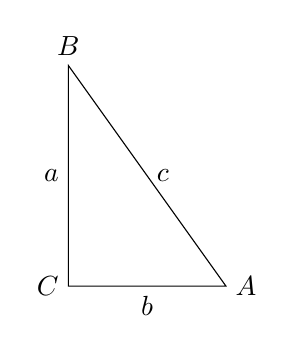
\begin{tikzpicture}
    % titik-titik segitiga
    \coordinate[label=left:$C$]  (C) at (-1.5cm,-1.cm);
    \coordinate[label=above:$B$] (B) at (-1.5cm,1.8cm);
    \coordinate[label=right:$A$] (A) at (0.5cm,-1.cm);
    
    % pembuatan segitiga
    \draw (A) -- node[right]{$c$} (B)  -- node[left]{$a$} (C) -- node[below]{$b$} cycle;
    \end{tikzpicture}
\end{center}

\subsection{Trigon}
\subsubsection{Rumus-rumus umum}
\begin{enumerate}
    \item $\sin (-x) = -\sin x$.
    \item $\cos (-x) = \cos x$.
    \item $\tan(-x) = -\tan x$.
    \item $\sin^2 x + \cos^2 x = 1$.
    \item $\sin(90^\circ-x)=\sin(90^\circ+x)=\cos x$.
    \item $\sin(a \pm b) = \sin a \cos b \pm \cos a \sin b$.
    \item $\sin 2x = 2\sin x \cos x$.
    \item $\cos(a \pm b) = \cos a \cos b \mp \sin a \sin b$.
    \item $\cos 2x = \cos^2 x - \sin^2 x = 2\cos^2 x -1 = 1-2\sin^2 x$.
    \item $\tan(a \pm b) = \dfrac{\tan a \pm \tan b}{1 \mp \tan a \tan b}$.
\end{enumerate}

\subsubsection{Dalil Sinus dan Dalil Cosinus}
\begin{center}
    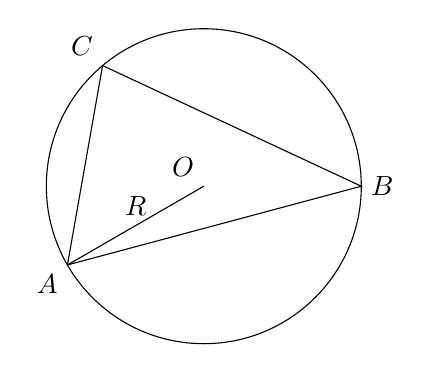
\begin{tikzpicture}
    \coordinate (O) at (0,0);
    \coordinate (B) at (0:2cm);
    \coordinate (A) at (210:2cm);
    \coordinate (C) at (130:2cm);
    
    \draw (O) circle (2cm);
    \draw (A) -- (B) -- (C) -- cycle;
    \node[right] at (B) {$B$};
    \node[below left] at (A) {$A$};
    \node[above left] at (C) {$C$};
    \node[above left] at (O) {$O$};
    \draw (A) -- node[above]{$R$} (O);
    \end{tikzpicture}
\end{center}
    \subsubsection{Dalil Sinus}
    $$\dfrac{BC}{\sin \angle A} = \dfrac{CA}{\sin \angle B}= \dfrac{AB}{\sin \angle C} = 2R$$
    
    \subsubsection{Dalil Cosinus}
    \begin{align*}
        AB^2 &= BC^2 + CA^2 - 2\cdot BC \cdot CA \cdot \cos \angle C\\
        BC^2 &= CA^2 + AB^2 - 2\cdot CA \cdot AB \cdot \cos \angle A\\
        CA^2 &= AB^2 + BC^2 - 2\cdot AB \cdot BC \cdot \cos \angle B
    \end{align*}

\subsection{Dalil Stewart}
    Pada segitiga $ABC$ dengan titik $D$ pada segmen $BC$, dimana $AB=c, BC=a, CA=b, AD=d, BD=m, CD=n$, maka berlaku
    \begin{align*}
        BC \cdot AD^2 + BC \cdot BD \cdot CD &= CA^2 \cdot BD + AB^2 \cdot CD\\
        ad^2+amn &= b^2m+c^2n
    \end{align*}
\begin{center}
    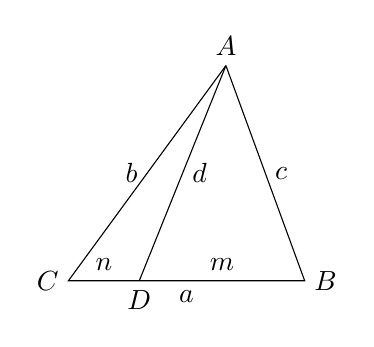
\begin{tikzpicture}
    % titik-titik segitiga
    \coordinate[label=left:$C$]  (C) at (-1.5cm,-1.cm);
    \coordinate[label=right:$B$] (B) at (1.5cm,-1.0cm);
    \coordinate[label=above:$A$] (A) at (0.5cm,1.732cm);
    % titik-titik cevian
    \coordinate[label=below:$D$] (D) at ($(C)!0.3!(B)$);
    
    % pembuatan segitiga
    \draw (A) -- node[right]{$c$} (B) -- node[above]{$m$} (D) -- node[above]{$n$} (C) -- node[left]{$b$} (A);
    
    
    % pembuatan cevian
    \draw (B) --node[below]{$a$}(C);
    \draw (A) --node[right]{$d$}(D);
    \end{tikzpicture}
\end{center}

\subsection{Teorema Garis Bagi}
Misalkan garis bagi sudut $\angle A$ (bisa garis bagi dalam atau garis bagi luar) memotong garis $BC$ di $K$, maka 
$$\dfrac{BK}{CK} = \dfrac{AB}{AC}.$$
\begin{center}
    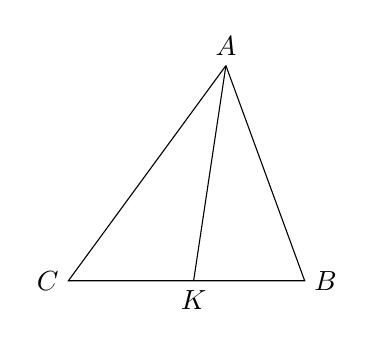
\begin{tikzpicture}
    % titik-titik segitiga
    \coordinate[label=left:$C$]  (C) at (-1.5cm,-1.cm);
    \coordinate[label=right:$B$] (B) at (1.5cm,-1.0cm);
    \coordinate[label=above:$A$] (A) at (0.5cm,1.732cm);
    % titik-titik cevian
    \coordinate[label=below:$K$] (D) at ($(C)!0.53!(B)$);
    
    % pembuatan segitiga
    \draw (A) --  (B) -- (D) -- (C) -- (A);
    
    
    % pembuatan cevian
    \draw (A) -- (D);
    \end{tikzpicture}
\end{center}


\subsection{Dalil Ceva}
Jika pada segitiga $ABC$, titik $D,E,F$ berturut-turut berada di segmen $BC$,$CA$,$AB$, maka 
$AD,BE,CF$ konkuren atau berpotongan di satu titik jika dan hanya jika $$\dfrac{AF}{FB} \cdot \dfrac{BD}{DC} \cdot \dfrac{CE}{EA} = 1.$$
\begin{center}
    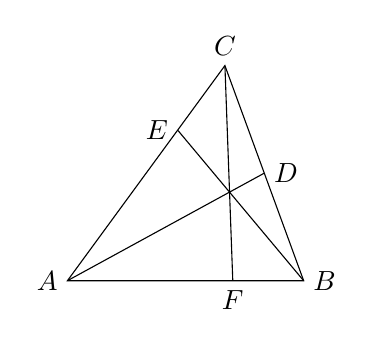
\begin{tikzpicture}
    % titik-titik segitiga
    \coordinate[label=left:$A$]  (A) at (-1.5cm,-1.cm);
    \coordinate[label=right:$B$] (B) at (1.5cm,-1.0cm);
    \coordinate[label=above:$C$] (C) at (0.5cm,1.732cm);
    
    % pembuatan segitiga
    \draw (A) -- (B) -- (C) -- cycle;
    
    % titik-titik cevian
    \coordinate[label=below:$F$] (F) at ($(A)!0.7!(B)$);
    \coordinate[label=right:$D$] (D) at ($(B)!0.5!(C)$);
    \coordinate[label=left:$E$]  (E) at ($(C)!0.3!(A)$);
    
    % pembuatan cevian
    \draw (A) -- (D);
    \draw (B) -- (E);
    \draw (C) -- (F);
    \end{tikzpicture}
\end{center}

\subsection{Dalil Menelaus}
Jika pada segitiga $ABC$, titik $P,Q,R$ berturut-turut berada pada garis (bisa di perpanjangan segmen) $BC$,$CA$, $AB$, maka $P,Q,R$ segaris jika dan hanya jika
$$\dfrac{AR}{RB} \cdot \dfrac{BP}{PC} \cdot \dfrac{CQ}{QA} = 1.$$
\begin{center}
    \begin{asy}
        unitsize(10);
        defaultpen(fontsize(8));
        pair P=(7,6), Q=(0,0), C=(10,0), A=(4,0), B=(6,8), R;
        draw((A)--(B)--(C)--cycle,blue+0.75);
        draw(P--R--Q--A);
        R=intersectionpoint(A--B,Q--P);
        dot(A^^B^^C^^P^^Q^^R);
        label("A",A,(0,-1));label("B",B,(1,0));label("C",C,(1,0));label("P",P,(1,1));label("Q",Q,(-1,0));label("R",R,(-1,1));
    \end{asy}
\end{center}

\subsection{Lingkaran}
\subsubsection{Berhubungan dengan Luas}
\begin{enumerate}
    \item $[ABC]=\sqrt{s(s-a)(s-b)(s-c)}$.
    \item $r=\dfrac{[ABC]}{s}$.
    \item $[ABC]=\dfrac{abc}{4R}$
\end{enumerate}

\subsubsection{Dalil Ptolemy}
    Diketahui sebuah segiempat siklis $ABCD$ maka berlaku
    $$AB \cdot CD + BC \cdot DA = AC \cdot BD.$$

\begin{center}
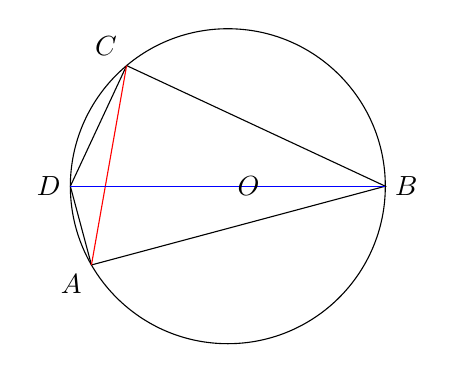
\begin{tikzpicture}
\coordinate (O) at (0,0);
\coordinate (B) at (0:2cm);
\coordinate (A) at (210:2cm);
\coordinate (D) at (180:2cm);
\coordinate (C) at (130:2cm);

\draw (O) circle (2cm);

\draw (A) -- (B) -- (C) -- (D) -- cycle;
\draw[red] (A) -- (C);
\draw[blue] (B) -- (D);

\node[right] at (B) {$B$};
\node[below left] at (A) {$A$};
\node[left] at (D) {$D$};
\node[above left] at (C) {$C$};
\node[right] at (O) {$O$};
\end{tikzpicture}
\end{center}

\subsubsection{Power of a Point}
\begin{figure}[h]
  \begin{asy}
    unitsize(1.5cm);
    pair O, A, B, C, D, E, P;
    O = (0,0);
    P = (4,1);
    E = (0,1);
    A = dir(50);
    C = dir(-30);
    circle o = circumcircle(A,E,C);
    draw(o);
    pair B1[] = intersectionpoints(line(A,P), o);
    pair D1[] = intersectionpoints(line(C,P), o);
    B = B1[0];
    D = D1[0];
    draw(A--B);
    draw(C--D);
    draw(P--A);
    draw(P--D);
    draw(P--E, red);
    draw(P--O, blue+dotted);
    label("$O$",O,SW);
    label("$A$",A,E);
    label("$B$",B,N);
    label("$C$",C,SE);
    label("$D$",D,SW);
    label("$P$",P,NE);
    label("$E$",E,N);
    \end{asy}
    \begin{asy}
    unitsize(1.5cm);
    pair O, A, B, C, D, P;
    O = (0,0);
    A = dir(50);
    C = dir(130);
    D = dir(-30);
    B = dir(-110);
    P = extension(A,B,C,D);
    draw(circumcircle(A,B,C));
    draw(A--B);
    draw(C--D);
    draw(A--C--B--D--cycle);
    draw(O--P, dotted);
    label("$O$",O,SW);
    label("$A$",A,E);
    label("$B$",B,SW);
    label("$C$",C,NW);
    label("$D$",D,SE);
    label("$P$",P,E);
    \end{asy}
\end{figure}
Diberikan lingkaran $\Gamma$ dan titik $P$ yang terletak di dalam atau di luar lingkaran $\Gamma$. Maka definisikan kuasa atau power dari $P$ terhadap lingkaran $\Gamma$ sebagai
$$Pow_\Gamma (P) = |OP^2-r^2|$$
dimana $O$ adalah pusat dari $\Gamma$ dan $r$ adalah jari-jari lingkaran $\Gamma$.

Jika $A,B,C,D$ berada di $\Gamma$, serta $AB$ dan $CD$ berpotongan di $P$, maka $$Pow_\Gamma(P)=PA \cdot PB = PC \cdot PD.$$
Jika $P$ berada di luar $\Gamma$ dan $E$ berada di $\Gamma$ sehingga $PE$ bersinggungan dengan $\Gamma$ di $E$, maka $$Pow_\Gamma (P) = PE^2 =  PA \cdot PB = PC \cdot PD.$$

\subsubsection{Euler's Theorem}
Rumusnya aja yah: $OI^2=R^2-2Rr$. Intinya diturunin pake Power of A Point.

\section{Analit Tidak Suci: Coordinate Bashing}
Tidak semua, tapi cukup banyak rumus:
\begin{itemize}
    \item Persamaan garis yang menghubungkan titik $(x_1, y_1)$ dan titik $(x_2, y_2)$:
    \[ y - y_1 = m(x - x_1) \quad \text{dimana} \quad m = \frac{y_2 - y_1}{x_2 - x_1} \text{ adalah kemiringan garis.} \]
    
    \item Jarak antara titik $(x_1, y_1)$ dan $(x_2, y_2)$:
    \[ d = \sqrt{(x_2 - x_1)^2 + (y_2 - y_1)^2} \]
    
    \item Titik tengah antara dua titik $(x_1, y_1)$ dan $(x_2, y_2)$:
    \[ M = \left(\frac{x_1 + x_2}{2}, \frac{y_1 + y_2}{2}\right) \]
    
    \item Persamaan lingkaran dengan radius $r$ dan pusat $(a, b)$:
    \[ (x - a)^2 + (y - b)^2 = r^2 \]
    
    \item Formula untuk garis tegak lurus
    \[ m_1m_2 = -1, \quad \text{dimana } m_1, m_2 \text{ adalah kemiringan dari dua garis yang saling tegak lurus.} \]
    
    \item Kemiringan sebuah garis yang melalui titik asal $O$:
    \[ m = \tan(\theta) \quad \text{dimana } \theta \text{ adalah sudut yang dibentuk garis dengan sumbu x.} \]
    
    \item Luas segitiga dari koordinat $(x_1, y_1)$, $(x_2, y_2)$, $(x_3, y_3)$:
    \[ A = \frac{1}{2} 
    \left| 
    x_1(y_2 - y_3) + x_2(y_3 - y_1) + x_3(y_1 - y_2) 
    \right| \]
\end{itemize}


\section{Soal Latihan}
\begin{enumerate}
    \item (OSN 2003) Diketahui segitiga $ABC$ siku-siku di $C$ dengan panjang sisi-sisinya merupakan bilangan bulat. Tentukan panjang sisi-sisi segitiga tersebut jika hasil kali dari dua sisi yang bukan sisi miring sama dengan tiga kali keliling segitiga.

    \item (OSN 2005) Misalkan $M$ suatu titik di dalam segitiga $ABC$ sedemikian rupa hingga $\angle AMC = 90^\circ$, $\angle AMB = 150^\circ$ dan $\angle BMC = 120^\circ$. Titik pusat lingkaran luar dari segitiga-segitiga $AMC$, $AMB$ dan $BMC$ berturut-turut adalah $P$, $Q$ dan $R$. Buktikan bahwa luas segitiga $PQR$ lebih besar dari luas segitiga $ABC$.

    \item (OSN 2006) Misalkan $S$ adalah himpunan semua segitiga $ABC$ yang memenuhi sifat: $\tan A$, $\tan B$ dan $\tan C$ adalah bilangan-bilangan asli. Buktikan bahwa semua segitiga anggota $S$ sebangun.

    \item (OSN 2008) Diberikan segitiga $ABC$ dengan panjang sisi-sisinya $a$, $b$, dan $c$. Garis-garis singgung lingkaran dalam segitiga $ABC$ yang sejajar dengan sisi-sisi segitiga $ABC$ membentuk tiga segitiga kecil. Pada masing-masing segitiga kecil dibuat lingkaran dalam. Buktikan bahwa jumlah luas dari lingkaran dalam segitiga $ABC$ dan ketiga lingkaran dalam segitiga kecil adalah
    \[\frac{\pi(a^2 + b^2 + c^2)(b + c - a)(c + a - b)(a + b - c)}{(a + b + c)^3}\]

    \item (OSN 2011) Diberikan sebarang segitiga lancip $ABC$. Misalkan $\ell_a$ garis yang melalui $A$ dan tegak lurus $AB$, $\ell_b$ garis yang melalui $B$ dan tegak lurus $BC$, $\ell_c$ garis yang melalui $C$ dan tegak lurus $CA$. Misalkan garis $\ell_b$ dan $\ell_c$ berpotongan di titik $D$, garis $\ell_c$ dan $\ell_a$ berpotongan di titik $E$ dan terakhir garis $\ell_a$ dan $\ell_b$ berpotongan di titik $F$. Buktikan bahwa luas segitiga $DEF$ paling sedikit tiga kali luas segitiga $ABC$.

    \item (OSN 2013) Diberikan segitiga lancip $ABC$ dengan lingkaran luar $\omega$. Garis bagi $\angle BAC$ memotong $\omega$ di titik $M$. Misalkan $P$ suatu titik pada garis $AM$ dengan $P$ di dalam segitiga $ABC$. Garis melalui $P$ yang sejajar $AB$ dan garis melalui $P$ yang sejajar $AC$ memotong sisi $BC$ berturut-turut di titik $E$ dan $F$. Garis $ME$ dan $MF$ memotong $\omega$ lagi berturut-turut di titik $K$ dan $L$. Buktikan bahwa garis-garis $AM$, $BL$ dan $CK$ konkuren.

    \item (OSN 2014) Diberikan trapesium $ABCD$ dengan $AB$ sejajar $CD$ dan $AB < CD$. Misalkan diagonal $AC$ dan $BD$ bertemu di $E$ dan misalkan garis $AD$ dan $BC$ bertemu di titik $F$. Bangun jajar genjang $AEDK$ dan $BECL$. Buktikan bahwa garis $EF$ melalui titik tengah segmen $KL$.

    \item (OSN SL 2010) Pada segitiga $ABC$, misalkan $D$ adalah titik tengah $BC$, dan $BE$, $CF$ adalah garis tinggi. Buktikan bahwa $DE$ dan $DF$ keduanya adalah garis singgung lingkaran luar $\triangle AEF$. %(OSN SL 2010) 

\end{enumerate}


\end{document}
